\section{Question 1}
\textit{Estimate the natural frequency of the system by determining the motor frequency that results in the largest measured displacement amplitude.}

The main results are shown in Table \ref{tab:main_results}. The full dataset is shown in Table \ref{tab:frequency_response} in Appendix \ref{sec:sample_calculations}.
\begin{table}[H]
    \centering
    \caption{Main results for the forced damped SDOF vibration experiment}
    \label{tab:main_results}
    \begin{tabular}{cccc}
        \toprule
        Dataset \# & Frequency, $f$ & Displacement Amplitude, $\mathbb{X}$ & $\omega/p$ \\
        & (Hz) & (m) & \\
        \midrule
        1 & 4.141 & 2.91E-04 & 0.792 \\
        2 & 2.840 & 4.74E-04 & 0.543 \\
        3 & 2.923 & 5.87E-04 & 0.559 \\
        4 & 3.976 & 5.03E-04 & 0.760 \\
        5 & 4.733 & 3.82E-04 & 0.905 \\
        6 & 4.518 & 7.37E-04 & 0.864 \\
        7 & \textbf{5.231} & \textbf{1.98E-03} & 1.000 \\
        8 & 5.847 & 6.39E-04 & 1.118 \\
        9 & 6.626 & 4.51E-04 & 1.267 \\
        10 & 11.044 & 1.99E-04 & 2.111 \\
        11 & 12.424 & 1.93E-04 & 2.375 \\
        12 & 11.044 & 2.85E-04 & 2.111 \\
        13 & 12.424 & 2.32E-04 & 2.375 \\
        14 & 14.199 & 2.16E-04 & 2.714 \\
        \bottomrule
    \end{tabular}
\end{table}
From Table \ref{tab:main_results}, the largest measured displacement amplitude was 0.00198m, which occurs at a motor frequency of $\boxed{5.23 \text{Hz}}$.

\section{Question 2}
\textit{Plot $\mathbb{X}$ vs. $\omega/p$ to obtain the frequency response curve of the system.}

The data from Table \ref{tab:frequency_response} was plotted using Matplotlib in Python \cite{matplotlib}. The plot is shown in Figure \ref{fig:frequency_response_curve}. 
\begin{figure}[H]
    \centering
    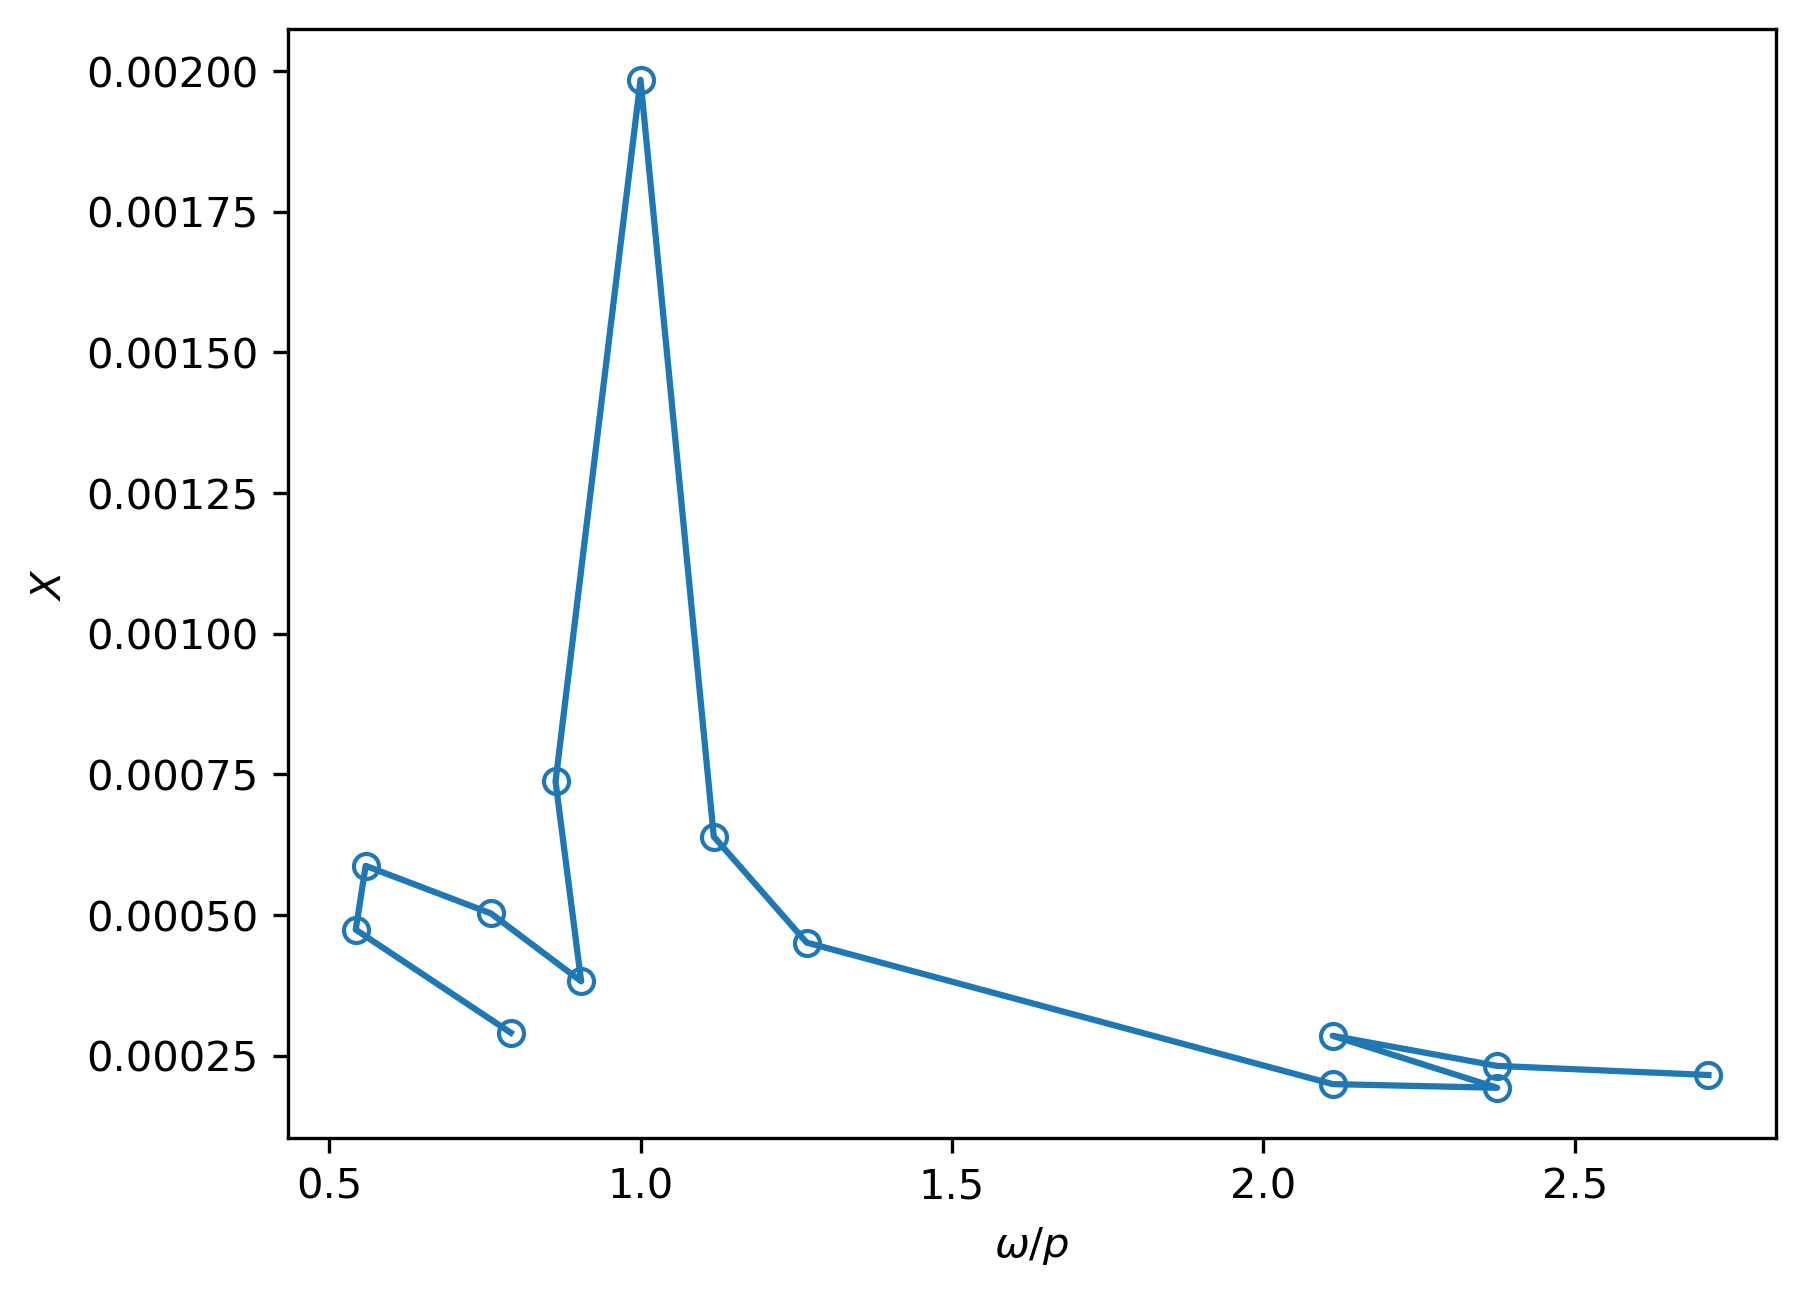
\includegraphics[width=0.8\textwidth]{Questions/Plots/X_vs_omega_p.png}
    \caption{Amplitude vs. $\omega/p$ Response Curve}
    \label{fig:frequency_response_curve}
\end{figure}

\section{Question 3}
\textit{Using your plot of $\mathbb{X}$ vs. $\omega/p$, estimate the damping ratio using the half-power bandwidth method. $\omega_1$ and $\omega_2$ can be determined using linear interpolation.}

\begin{figure}[h]
    \centering
    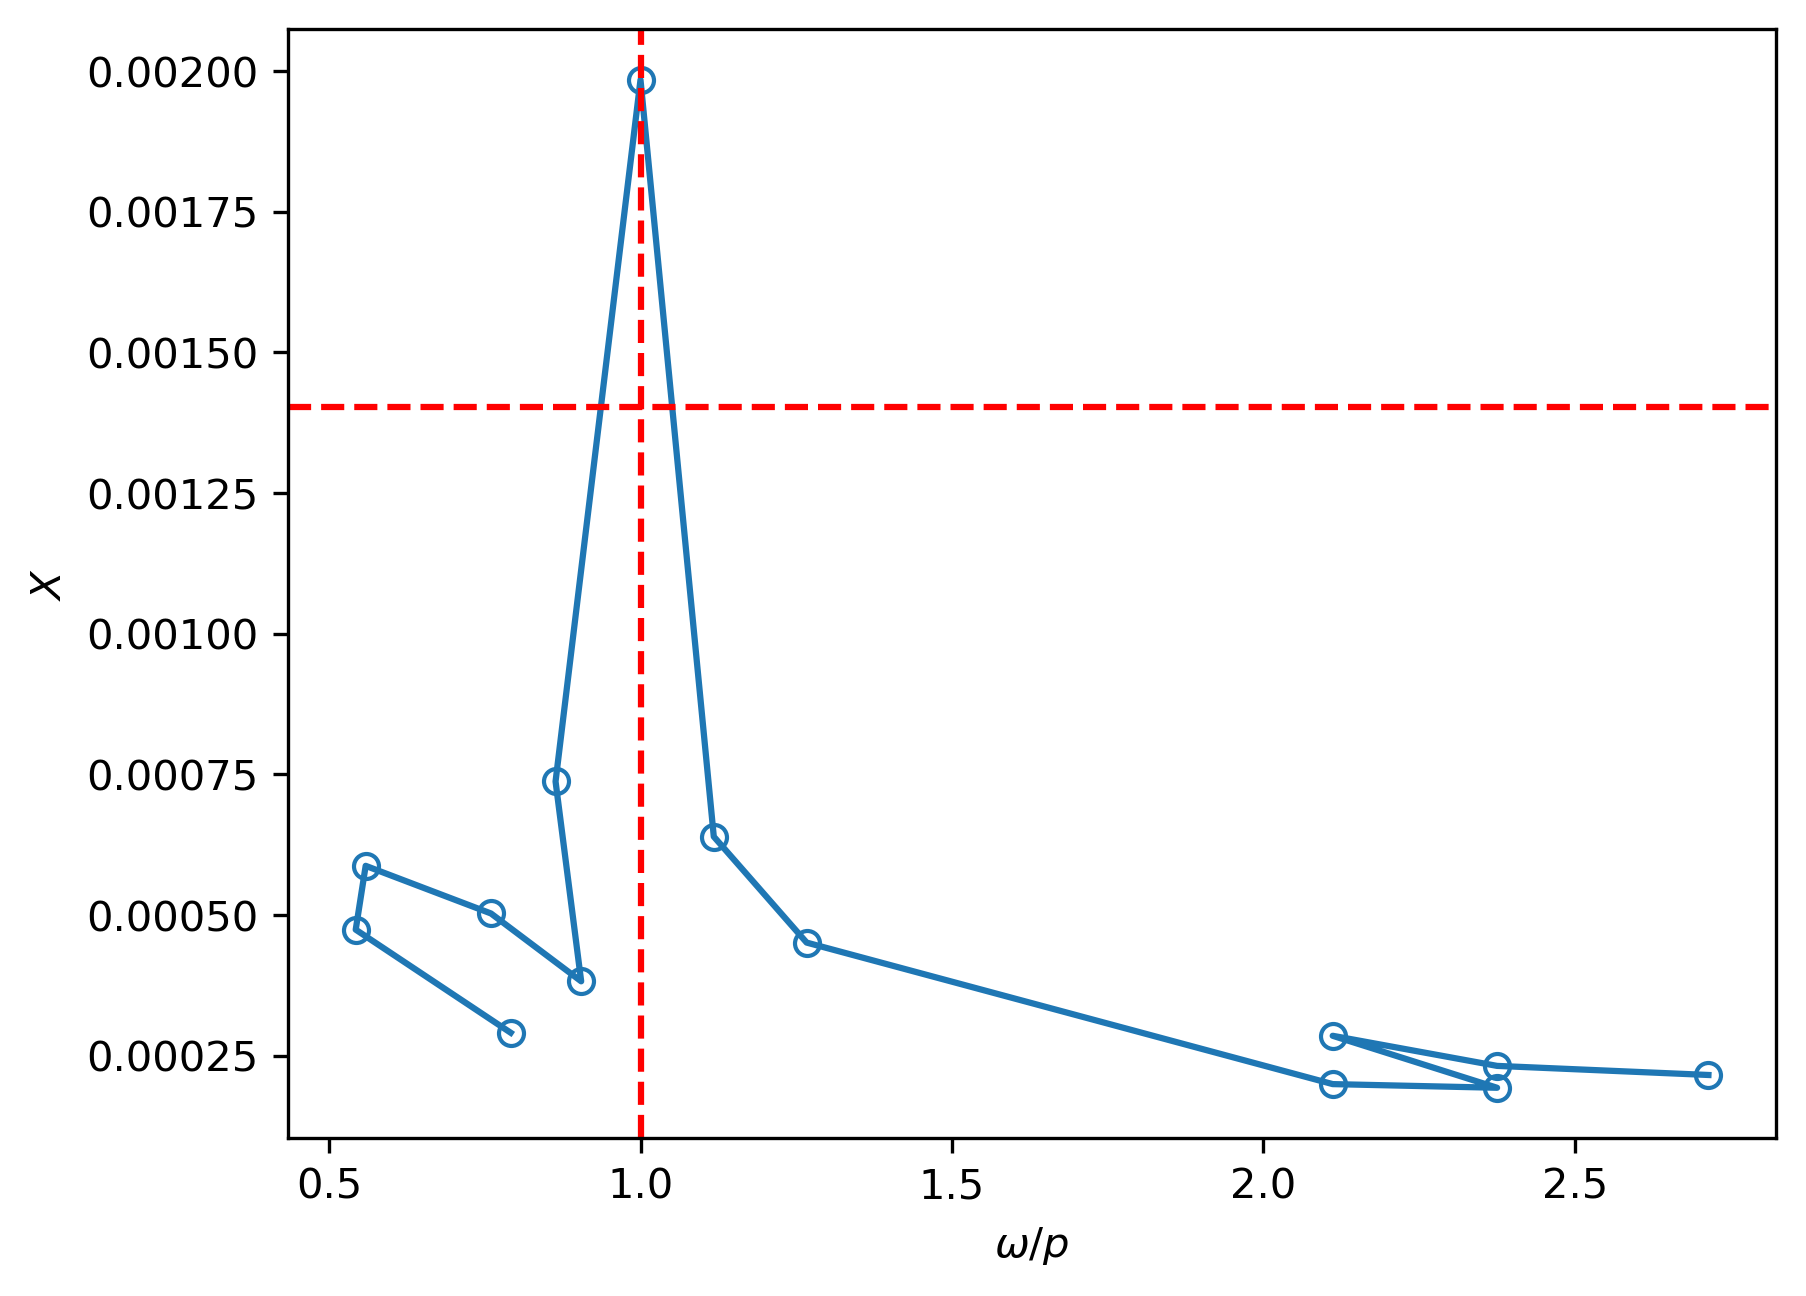
\includegraphics[width=0.8\textwidth]{Questions/Plots/X_vs_omega_p_with_lines.png}
    \caption{Annotated Amplitude vs. $\omega/p$ Response Curve}
    \label{fig:frequency_response_curve_with_lines}
\end{figure}
From the annotated frequency response curve in Figure \ref{fig:frequency_response_curve_with_lines}, the half-power bandwidth method was used to estimate the damping ratio. From linear interpolation of the LHS of the peak, denoting ($x$, $y$) = ($\omega/p$, $\mathbb{X}$), 
\begin{align*}
    x_{\text{LHS}} &= \frac{x_1 - x_2}{y_1 - y_2} \left(\frac{y_1}{\sqrt{2}} - y_1\right) + x_1 \\
    &= \frac{1 - 0.864}{0.00198 - 0.000737} \left(\frac{0.00198}{\sqrt{2}} - 0.00198\right) + 1 \\
    &= 0.9364 
\end{align*}
For the RHS of the peak,
\begin{align*}
    x_{\text{RHS}} &= \frac{x_1 - x_2}{y_1 - y_2} \left(\frac{y_1}{\sqrt{2}} - y_1\right) + x_1 \\
    &= \frac{1 - 1.118}{0.00198 - 0.000639} \left(\frac{0.00198}{\sqrt{2}} - 0.00198\right) + 1 \\
    &= 1.0508
\end{align*}
Then by the half-power bandwidth method, the damping ratio, $\zeta$, was calculated by
\begin{align*}
    \zeta = \frac{\omega_2 - \omega_1}{2p} &= \frac{\omega_{\text{RHS}}/p - \omega_{\text{LHS}}/p}{2} \\
    &= \frac{1.0508 - 0.9364}{2} \\
    &= \boxed{0.0572}
\end{align*}

\section{Question 4}
\textit{Using your calculated damping ratio, estimate the mass of a single imbalance (remember that there are two imbalances, not one), if they each have an eccentricity of 25 mm. Assume the total mass of the system is 13 kg.}

From Eq. (5.22),
\begin{align*}
    \frac{M \mathbb{X}}{\tilde{m}e} &= \frac{\left(\frac{\omega}{p}\right)^2}{\sqrt{\left[1 - \left(\frac{\omega}{p}\right)^2\right]^2 + \left(2\zeta\frac{\omega}{p}\right)^2}} 
\end{align*}
Rearranging,
\begin{align*}
    \tilde{m} &= \frac{M \mathbb{X}}{e} \frac{\sqrt{\left[1 - \left(\frac{\omega}{p}\right)^2\right]^2 + \left(2\zeta\frac{\omega}{p}\right)^2}}{\left(\frac{\omega}{p}\right)^2} 
\end{align*}
Using Dataset \#7 from Table \ref{tab:frequency_response}, 
\begin{align*}
    \tilde{m} &= \frac{13 \times 1.98 \times 10^{-3}}{0.025} \frac{\sqrt{\left[1 - \left(1\right)^2\right]^2 + \left(2 \times 0.0572 \times 1\right)^2}}{\left(1\right)^2} \\
    &= 0.11778624 \text{ kg}
\end{align*}
Since there are two imbalances, the mass of a single imbalance is 
\begin{align*}
    \boxed{\tilde{m}_{\text{single}} = 0.0589 \text{ kg}}
\end{align*}

\section{Question 5}
\textit{Estimate the natural frequency of the system using the vertical acceleration data recorded during beating of the platform and the motor frequency measured with the stroboscope.}

% The beating results are shown in Table \ref{tab:beating_results}. The maximum, minimum, and times were determined by inspection. The frequency was calculated by
% \begin{align*}
%     f_{\text{Phyphox}} &= \frac{1}{2(t_{\text{min}} - t_{\text{max}})} \\
%     &= \frac{1}{2(3.249 - 3.349)} \\
%     &= \boxed{4.969 \text{ Hz}}
% \end{align*}

% The natural frequency was also determined by stroboscope to be 
% \begin{align*}
%     f_{\text{Stroboscope}} &= \boxed{5 \text{ Hz}}
% \end{align*}

The period was determined from the beating results to be 
\begin{align*}
    \tau_b &= t_{\text{node1}} - t_{\text{node2}} \\
    &= 3.87756 - 2.77582 \\
    &= 1.10174 \text{ s}
\end{align*}
From the TA announcement, the formula for the natural frequency is given by
\begin{align*}
    \tau_b &= \frac{2\pi}{\omega - p} \\
\end{align*}
From using the stroboscope, the motor frequency was determined to be $f = 5 \text{ Hz}$. Then,
\begin{align*}
    \omega &= 2\pi f \\
    &= 2\pi \times 5 \\
    &= 31.416 \text{ rad/s}
\end{align*}
Then,
\begin{align*}
    p &= \omega - \frac{2\pi}{\tau} \\
    &= 31.416 - \frac{2\pi}{1.10174} \\
    &= 31.416 - 5.694 \\
    &= 25.713 \text{ rad/s}
\end{align*}
Which is 
\begin{align*}
    f &= \frac{p}{2\pi} \\
    &= \frac{25.713}{2\pi} \\
    &= \boxed{4.09 \text{ Hz}}
\end{align*}